%===============================================
% Dokumentenkopf
%===============================================
\RequirePackage{ifluatex}		% Für Compilerunterscheidung
\RequirePackage{xcolor}			% wegen Farbmischung
\documentclass[ngerman, ignorenonframetext]{beamer}	
\usetheme{ACUAS}				% CD der FH-Aachen
\ifluatex

\usepackage{fontspec}

\defaultfontfeatures{Ligatures=TeX}

\else

\usepackage[utf8]{inputenc}

\usepackage[T1]{fontenc}
\fi

\usepackage[english]{babel}

\usepackage{graphicx}

\usepackage{float}

\usepackage[english]{fancyref}

%\usepackage{mathtools}
%\DeclarePairedDelimiter{\abs}{\lvert}{\rvert}

\usepackage{setspace}

\usepackage[backend=biber,
autolang=hyphen,
style=alphabetic,
citestyle=alphabetic,
giveninits=false
]{biblatex}

 		% Einstellungen und Pakete
\title[Crime Category Prediction of Cities]{Crime Category Prediction of Cities Using an Ensemble of Various Classifiers}
\author[Hambsch \and Nolden \and Ahring \and Peters] {
	Hardy Hambsch
	\and
	Marius Nolden
	\and
	Jessica Ahring
	\and
	Christian Peters
}
\addbibresource{../common/literatur.bib}	% Ort der Literaturdatenbank

%===============================================
% Dokumentenrumpf
%===============================================
\begin{document}
	\mode<all>
	\begin{frame}
	\maketitle					% ist in config 
	\end{frame}
	\section{Introduction}

In a time of limited resources regarding fighting crimes, we aim to predict the crime category of different
cities to provide additional guidance when distributing those resources. \\

\noindent To emphasize the influence of certain factors on the criminal rates of cities, we use different
classifiers to predict the criminal category (i.e. high, medium and low) the city falls into. The classifiers
employed are namely k-Nearest Neighbors, Decision Tree, Na\"ive Bayes Classifier and Neural Network.
After training each classifier on its own, the obtained models are combined into an ensemble, the decision of
which is based on a majority vote. This is done to achieve even better results. 

In order to evaluate the results, we use the common evaluation metrics e.g accuracy, recall, precision and
f-measure.

In the course of this research the open source data mining software WEKA is used to apply the algorithms to
the dataset.

\vspace*{\fill}

	\section{Dataset}

This research is based on real crime data which can be obtained from the Machine Learning
Repository\footnote{http://archive.ics.uci.edu/ml/datasets/Communities+and+Crime}.

From the 128 attributes the dataset provides, only the most significant features are chosen which are all
continuous in nature:

\begin{itemize}
	\setlength{\itemsep}{-2pt}
	\item population 
	\item mean people per household
	\item percentage of population that is african american
	\item percentage of population that is caucasian
	\item percentage of population that is of asian heritage 
	\item percentage of population that is of hispanic heritage
	\item percentage of population that is 16-24 in age
	\item percentage of population that is 65 and over in age 
	\item median household income
	\item percentage of people under the poverty level
	\item percentage of people 25 and over with less than a 9th grade education 
	\item percentage of people 16 and over, in the labor force, and unemployed 
	\item percentage of population who are divorced
	\item percent of people who do not speak English well 
	\item population density in persons per square mile
	\item total number of violent crimes per 100K population 
\end{itemize}

The goal is to predict the crime category, which is an
\textit{artificial}\footnote{this attribute is added by us}, discrete and ordinal attribute.
The values of this attributes, i.e.
the classes that are to be predicted, are obtained by clustering the attribute "total number of violent
crimes per 100K population" into three labels: "high", "medium" and "low". To accomplish this, we use an
unsupervised learning approach, namely k-Means clustering.

For predicting the "crime category", the attribute "total number of violent crimes per 100K population" is
removed from the dataset, because it is already represented by the class division and would harm the ability
of the classifier to draw conclusions from other relevant attributes.

	\section{Literature Review}
	\mode*

\begin{frame}
	\section{Data Preparation}
	\frametitle{Data Preparation}
	\onslide<+->
        \begin{itemize}
          \item<+-> Before the classification can be done, a few steps are required on the raw data
          \item<+-> Original dataset does not contain the class labels ("High", "Medium", "Low")
            \begin{itemize}
              \item<+-> How to assign each instance a crime category based on its crime rate?
              \item<+-> How to find the percentage boundaries between the classes?
            \end{itemize}
          \item<+-> Curse of dimensionality
            \begin{itemize}
              \item<+-> Huge number of attributes (128 per city)
              \item<+-> Select only the most significant
              \item<+-> Reduce the dimensionality of the feature space
            \end{itemize}
        \end{itemize}
\end{frame}

\begin{frame}
  \frametitle{Assignment of Class Labels}
  \onslide<+->
  \begin{itemize}
    \item<+-> Divide the attribute "crime rate" into different groups
      \begin{itemize}
        \item<+-> Initial question: How many groups?
        \item<+-> What are the boundaries between the groups?
      \end{itemize}
    \item<+-> Use clustering to solve this problem
      \begin{itemize}
        \item<+-> Simple k-Means clustering algorithm
        \item<+-> Only cluster the crime rate (i.e. only one dimension)
        \item<+-> Test different k values (different amounts of groups)
        \item<+-> Find the boundaries between the groups
      \end{itemize}
    \item<+-> Each cluster will be assigned a label (e.g. "High", "Medium", "Low",\ldots crime rate)
  \end{itemize}
\end{frame}

\begin{frame}
  \frametitle{Assignment of Class Labels}
  \begin{figure}[H]
    \centering
    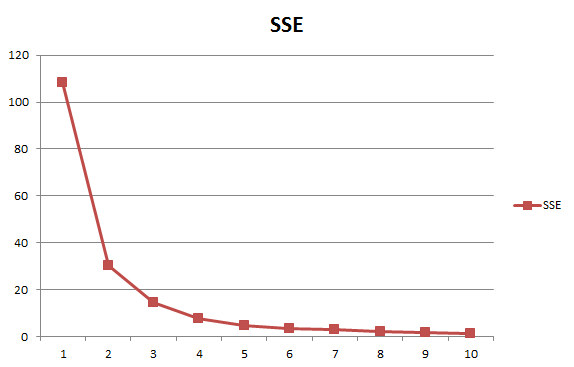
\includegraphics[width=0.8\columnwidth]{../../charts/SSE.png}
    \caption{Sum of the squared errors for different choices of k}
    \label{fig:sse}
  \end{figure}
\end{frame}

\begin{frame}
  \frametitle{Assignment of Class Labels}
  \onslide<+->
  \begin{itemize}
    \item<+-> By using the elbow-method, \(k=3\) is the best choice
      \begin{itemize}
        \item<+-> This means to divide the crime rate into three groups ("High", "Medium", "Low")
      \end{itemize}
    \item<+-> The percentage boundaries are extracted from the clusters
      \begin{itemize}
        \item<+-> Low: \([0\%; 22\%]\) 
	\item<+-> Medium: \((22\%; 56\%]\)
	\item<+-> High: \((56\%; 100\%]\)
      \end{itemize}
    \item<+-> Depending on the group it falls into, each instance (city) can now be assigned a label
  \end{itemize}
\end{frame}

\begin{frame}
  \frametitle{Feature Selection}
  \onslide<+->
  \begin {itemize}
    \item<+-> Two-step approach:
      \begin{enumerate}
        \item<+-> Create a ranking by judgement of significance
          \begin{itemize}
            \item<+-> Discuss each attribute
            \item<+-> Agree if it is included or not
          \end{itemize}
        \item<+-> Generate a ranking based on the correlation between each attribute and the class labels
      \end{enumerate}
    \item<+-> Compare the judgement ranking with the correlation ranking
    \item<+-> Add some features with high correlation and remove some with low correlation
      \begin{itemize}
        \item<+-> E.g. the attribute "population" was removed because of a correlation near zero
      \end{itemize}
  \end{itemize}
\end{frame}


Before the classification can be done, a few preparation steps are still
required, namely the assignment of class labels to each instance as
well as feature selection to reduce the set of attributes to an
acceptable size.

\subsection{Assignment of Class Labels}
\label{sec:assignment}

To obtain the class labels used for classification, the
continuous attribute "total number of violent crimes per 100K
population" is divided into separate groups. Each of this groups is
assigned an ordinal class label that can be predicted during classification.
If for example the number of groups is equal to three, one could
assign the labels "High", "Medium" and "Low" to the corresponding
groups.

The simple k-Means clustering algorithm is used to achieve this
by comparing different amounts of groups, i.e. testing
different values of k. Those different k values were compared by using
the elbow-method and \(k=3\) was revealed as the best parameter as
shown in \fref{fig:sse}.
\begin{figure}[H]
	\centering
	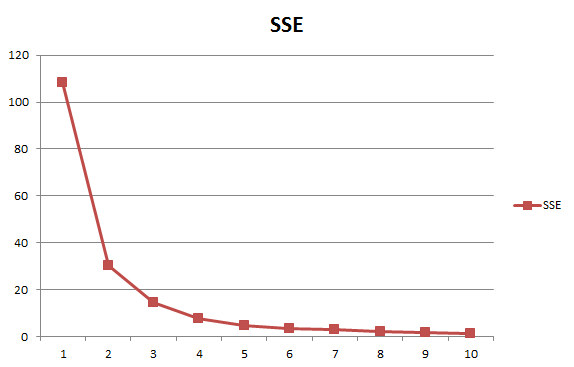
\includegraphics[width=\columnwidth]{../../charts/SSE.png}
	\caption{Sum of the squared errors for different choices of k}
	\label{fig:sse}
\end{figure}
\noindent The three classes originating from this choice are namely
"High", "Medium" and "Low", the percentage boundaries are
respectively:
\begin{description}
	\setlength{\itemsep}{-2pt}
	\item[Low:] \([0\%; 22\%]\) 
	\item[Medium:] \((22\%; 56\%]\)
	\item[High:] \((56\%; 100\%]\)
\end{description}
%% It should be noted, that the authors of \textit{"An Experimental Study
%% of Classification Algorithms for Crime Prediction"} \cite{indian}
%% obtained different results for the percentage boundaries, they did
%% however not disclose the details of their approach.
%% Their percentage boundaries are "Low": \([0\%;25\%)\), "Medium": \([25\%; 40\%)\) and "High": \([40\%; 100\%]\).

\subsection{Feature Selection}
\label{sec:feature_selection}    

To reduce the total of 128 attributes in the dataset to an acceptable
amount, we employed a two-step approach that is presented in the
following sections.

\paragraph{Selection by Judgement of Significance}
First we discussed each attribute separately and agreed whether we
would include it based on its significance. In the course of this
procedure, we obtained a ranking of the attributes we regarded as most
significant.

\paragraph{Comparison with Correlation Ranking}
In the second step, we compared our choices with the attributes that
have the highest correlation with the classes. We found that the
majority of the attributes that we selected based on common sense was
already present in the ranking, however a few attributes like
"population" were discarded because of a correlation near zero.


\mode<all>

	%\section{Clustering}
To optain the class labels used in the classification process, the simple k-Means clustering algorithm is applied to the attribute "total number of violent crimes per
100K population". By using the elbow-method to search for the most significant k, k equals three was revealed as the best parameter as shown in \fref{fig:sse}.
\begin{figure}[H]
	\centering
	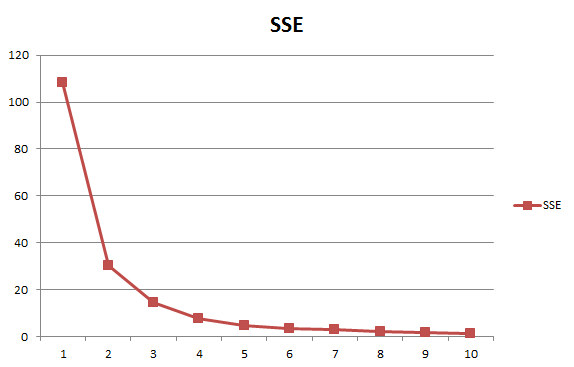
\includegraphics[width=\columnwidth]{../../charts/SSE.png}
	\caption{Sum of the squared errors for different choices of k}
	\label{fig:sse}
\end{figure}
The three classes originating from this choice are namely "High", "Medium" and "Low", the percentage boundaries are respectively:
\begin{description}
	\item[Low:] \([0\%; 22\%]\) 
	\item[Medium:] \((22\%; 56\%]\)
	\item[High:] \((56\%; 100\%]\)
\end{description}

It should be noted, that the authors of \textit{"An Experimental Study of Classification Algorithms for Crime Prediction"} \cite{indian} obtained different results for the percentage boundaries, they did however not disclose the details of their approach. Their percentage boundaries are "Low": \([0\%;25\%)\), "Medium": \([25\%; 40\%)\) and "High": \([40\%; 100\%]\).



	\section{Experimental Results}
The different approaches used for the classification purpose and the corresponding results are described in the following sections. 
\subsection{Approaches and Settings}

\subsubsection*{k-Nearest Neighbors}
The first approach we use is the k-Nearest Neighbors classifier. The parameter k is obtained by performing a parameter search on a leave-one-out cross validation. In terms of accuracy, k equals 16 was the best choice. To weight the different votes, inverse-distance weighting is employed, the distance measure is Manhattan Metric. 

\subsubsection*{Na\"ive Bayes}
Another approach is the Na\"ive Bayes classifier. Despite some attributes obviously not being independent, we still employed this classifier because it proved to be useful in other areas as well.  

\subsubsection*{Decision Tree}
We generated a pruned J48-decision tree. Using sparse parameter search for the confidence factor, we discovered that a tree with 33 nodes delivers the best results in terms of accuracy.

\subsubsection*{Neural Network}
A multilayer perceptron is used as a neural network. The structure consists of 15 input neurons (one for each attribute), a hidden layer of five neurons precedes the output layer containing three neurons (one for each class). A learning rate of 0.15 is used, a momentum of 0.075 is applied in each training step. 

\subsubsection*{Ensemble}
In hope for enhanced results by combining the strenghts of the different classifiers, all models are combined into an ensemble. The vote of the whole ensemble is found by conducting a majority voting. 

\subsection{Results}
To illustrate the accuracy of the different methods employed, the confusion matrices are presented here. All results are found using 10-fold cross validation.

The results of k-Nearest Neighbors are shown in \ref{tab:mat-knn}.

\begin{table}[H]
	\centering
	\caption{Confusion matrix of the k-Nearest Neighbors classifier with Manhattan distance}
	\label{tab:mat-knn}
	\resizebox{\columnwidth}{!}{
	\begin{tabular}[c]{c|ccc||c}
		classified \(\rightarrow\) & \textbf{Low} & \textbf{Medium} & \textbf{High} & Total\\ \hline
		Low & \textcolor{blue}{1155} & 101 & 3 & 1259 \\
		Medium & 181 & \textcolor{blue}{304} & 37 & 522 \\
		High & 21 & 112 & \textcolor{blue}{80} & 213 \\ \hline \hline
		Total & 1357 & 517 & 120 & 1994 \\
	\end{tabular}
}
\end{table}

The results of the Na\"ive Bayes classifier are shown in \fref{tab:mat-nb}.
\begin{table}[H]
	\centering
	\caption{Confusion matrix of the Na\"ive Bayes classifier}
	\label{tab:mat-nb}
	\resizebox{\columnwidth}{!}{
	\begin{tabular}[c]{c|ccc||c}
		classified \(\rightarrow\) & \textbf{Low} & \textbf{Medium} & \textbf{High} & Total\\ \hline
		Low & \textcolor{blue}{1063} & 183 & 13 & 1259 \\
		Medium & 137 & \textcolor{blue}{282} & 103 & 522 \\
		High & 15 & 68 & \textcolor{blue}{130} & 213 \\ \hline \hline
		Total & 1215 & 533 & 246 & 1994 \\
	\end{tabular}
}
\end{table}

The confusion matrix of the decision tree is illustrated in \fref{tab:mat-tree}.
\begin{table}[H]
	\centering
	\caption{Confusion matrix of the decision tree}
	\label{tab:mat-tree}
	\resizebox{\columnwidth}{!}{
	\begin{tabular}[c]{c|ccc||c}
		classified \(\rightarrow\) & \textbf{Low} & \textbf{Medium} & \textbf{High} & Total\\ \hline
		Low & \textcolor{blue}{1135} & 111 & 13 & 1259 \\
		Medium & 194 & \textcolor{blue}{277} & 51 & 522 \\
		High & 23 & 105 & \textcolor{blue}{85} & 213 \\ \hline \hline
		Total & 1352 & 493 & 149 & 1994 \\
	\end{tabular}
}
\end{table}

The results of the neural network classifier can be found in \fref{tab:mat-nn}.
\begin{table}[H]
	\centering
	\caption{Confusion matrix of the Neural Network}
	\label{tab:mat-nn}
	\resizebox{\columnwidth}{!}{
		\begin{tabular}[c]{c|ccc||c}
			classified \(\rightarrow\) & \textbf{Low} & \textbf{Medium} & \textbf{High} & Total\\ \hline
			Low & \textcolor{blue}{1128} & 128 & 3 & 1259 \\
			Medium & 168 & \textcolor{blue}{317} & 37 & 522 \\
			High & 12 & 108 & \textcolor{blue}{93} & 213 \\ \hline \hline
			Total & 1308 & 553 & 133 & 1994 \\
		\end{tabular}
	}
\end{table}

The confusion matrix containing the results of the majority voting is given in \fref{tab:mat-vote}.

\begin{table}[H]
	\centering
	\caption{Confusion matrix of the ensemble}
	\label{tab:mat-vote}
	\resizebox{\columnwidth}{!}{
		\begin{tabular}[c]{c|ccc||c}
			classified \(\rightarrow\) & \textbf{Low} & \textbf{Medium} & \textbf{High} & Total\\ \hline
			Low & \textcolor{blue}{1084} & 163 & 12 & 1259 \\
			Medium & 138 & \textcolor{blue}{295} & 89 & 522 \\
			High & 16 & 71 & \textcolor{blue}{126} & 213 \\ \hline \hline
			Total & 1238 & 529 & 227 & 1994 \\
		\end{tabular}
	}
\end{table}

An overview of the different evaluation metrics is presented in \fref{fig:result}.
\begin{figure}[H]
	\centering
	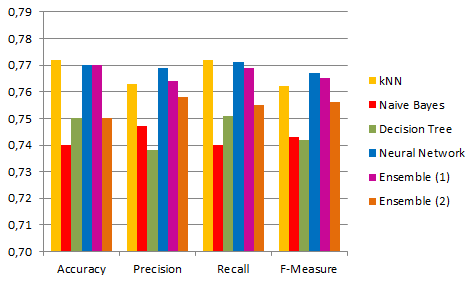
\includegraphics[width=\columnwidth]{../../charts/results.png}
	\caption{Evaluation metrics of the different classifiers}
	\label{fig:result}
\end{figure}

\begin{figure}[H]
	\centering
	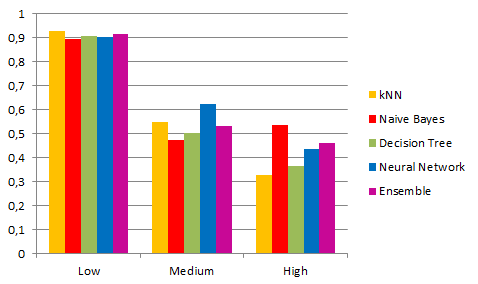
\includegraphics[width=\columnwidth]{../../charts/recall.png}
	\caption{Recall of the different classifiers}
	\label{fig:recall}
\end{figure}

\subsection{Discussion}

Considering all the evaluation metrics shown in \fref{fig:result}, the Neural Network delivered the best results in every case. Contrary to the initial believe that the majority voting would enhance the results, it turned out that they were merely average. 
 
To compare our results with those of \cite{indian}, it should be considered that on the one hand they used predefined ranges for their classification and on the other hand they used different attributes, mostly focusing on income and education.




    \begin{frame}
  \frametitle{Discussion an Outlook}
  \begin{itemize}
    \item Each classifier has its strengths and weaknesses
      \begin{itemize}
        \item k-Nearest Neighbors excels in accuracy and overall recall
        \item Neural Network scores best in terms of precision and f-measure
        \item Na\"ive Bayes has extraordinary recall with respect to class "High"
      \end{itemize}
    \item Contrary to what we initially thought -- the ensemble was merely average
      \begin{itemize}
        \item Always among the best
        \item Never reached top spot in any category
      \end{itemize}
    \item How can that be?
      \begin{itemize}
        \item Not only strengths are merged but weaknesses as well
        \item Strengths and weaknesses average out
      \end{itemize}
    \item Can this be improved?
      \begin{itemize}
        \item In our case, each base learner had an equal weight
        \item Improve the results by changing the weights
        \item Emphasize strengths of one classifier (e.g. high recall
          of Na\"ive Bayes), mitigate weaknesses of another
      \end{itemize}
  \end{itemize}
\end{frame}

\begin{frame}[c]
  \frametitle{Discussion and Outlook}
  \center
  \textbf{Thank you very much for listening!}
  
  \textbf{Any questions left?}
\end{frame}

	\begin{frame}[allowframebreaks] % Folien dürfen sich umbrechen
			\nocite{*}
			\printbibliography	% Literaturverzeichnis
	\end{frame}
	\mode*
\end{document}
